\normaltrue \difficilefalse \tdifficilefalse
\correctionfalse

%\UPSTIidClasse{11} % 11 sup, 12 spé
%\newcommand{\UPSTIidClasse}{12}
% ATS 2019
\exer{Pilote hydraulique de voilier$\star$ \label{A3:05:90}}
\setcounter{numques}{0}
\UPSTIcompetence[2]{A3-05}
\index{Compétence A3-05}
\index{Pilote hydraulique}
\index{Caractériser un constituant de la chaîne de puissance}
\index{Distributeur}
\index{Vérin}
\ifcorrection
\else
\textbf{Pas de corrigé pour cet exercice.}
\fi



\ifprof
\else
On s'intéresse à la distribution d'énergie hydraulique dans le pilote hydraulique de voilier. 

On donne se premier schéma hydraulique. L'énergie est distribuée par un distributeur monostable 2 positions, 2 orifices. 

\begin{center}
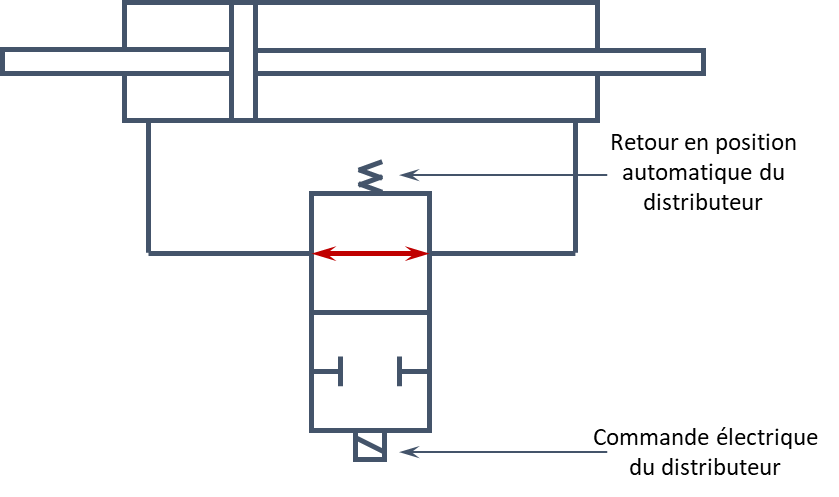
\includegraphics[width=\linewidth]{90_fig_01}
%\textit{}
\end{center}


\fi


\question{Le schéma précédent est donné dans la situation << au repos >>. Que se passe-t-il si l'utilisateur manipule le vérin à la main ?}
\ifprof
\begin{corrige}
L'huile peut circuler d'une chambre à l'autre en passant par le distributeur. Le vérin peut donc se translater.
\end{corrige}
\else
\fi

\question{On actionne le distributeur. Que se passe-t-il si l'utilisateur manipule le vérin à la main ?}
\ifprof
\begin{corrige}
Le distributeur bloque la circulation de l'huile. Le vérin est bloqué.
%\begin{center}
%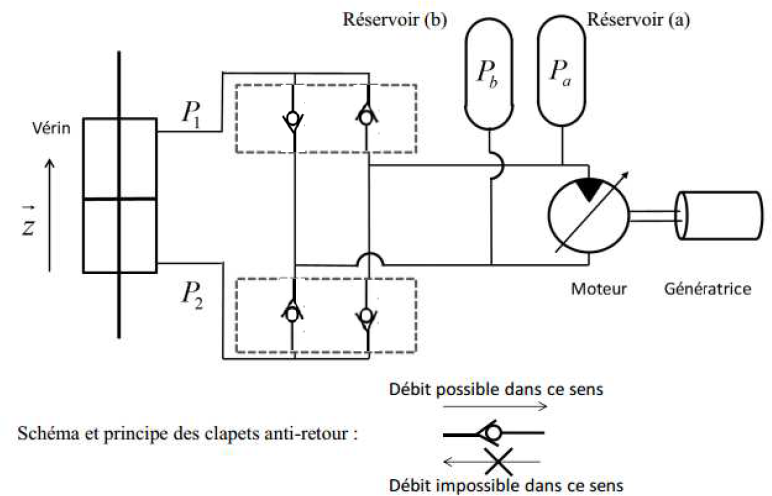
\includegraphics[width=.5\linewidth]{89_cor_01}
%\textit{}
%\end{center}
\end{corrige}
\else
\fi

\ifprof
\else
\begin{flushright}
\footnotesize{Corrigé  voir \ref{A3:05:90}.}
\end{flushright}%
\fi